\documentclass[a4paper,12pt]{article}

\usepackage{microtype}
\usepackage{biblatex}
\usepackage{hyperref}
\usepackage{graphicx}
\usepackage{amsmath}

\addbibresource{paper.bib}

\title{Simulating an Interplanetary Internet}
\author{Cody Auch, Jacob Janzen, Mark Lysack}
\date{\today}

\newcommand{\CC}{C\nolinebreak\hspace{-.05em}\raisebox{.4ex}{\tiny\bf
    +}\nolinebreak\hspace{-.10em}\raisebox{.4ex}{\tiny\bf +}}
\def\CC{{C\nolinebreak[4]\hspace{-.05em}\raisebox{.4ex}{\tiny\bf ++}}}

\begin{document}
\maketitle

\begin{abstract}
  This paper discusses interplanetary networks, the challenges that can arise
  from them that make them a unique challenge compared to shorter-range computer
  networks, and how our current network protocols can be applied in this
  application. In addition, we look at how one can use conventional network
  simulators to test interplanetary network implementations. We used the network
  simulator NS-3~\cite{ns-3} to test various transport layer protocols against
  each other in a network topology that we designed in the network simulator to
  emulate long-distance communications. Using this network simulation, we were
  able to compare UDP, TCP, and TCP New Reno protocols against each other to see
  how they each performed across such large distances with high delays. UDP
  preformed the best with New Reno and TCP closely paired together.

  Our implementation can be found
  at \url{https://github.com/codyauch/IPN-Project}. The physics simulation was
  mostly designed by Mark and Cody. The network simulation in NS-3 was done by
  Jacob, and the analysis was done by Mark.
\end{abstract}

\section{Introduction}

In the past decade interest in returning back to space has increased
internationally. Many organizations have started sending remote vehicles into
space for the first time~%\cite{(indian space program, spaceX, ect)}
and there are talks of a permanent lunar base being created. With an increased
amount of satellites and potentially permanent bases outside of Earths orbit,
the demand on the interplanetary network (IPN) is increased. The IPN has a
series of unique challenges such as a high amount of error, constantly changing
network topology, and long propagation delay. The solution to these problems is
implementing a delay tolerant network. While space organizations have maintained
the IPN with a set of standard protocols, these may not be sufficient for an
expanding network. The simulator proposed shows how an IPN can handle different
stages of development of an IPN as well as increased throughput requirements.
Before these technological changes can be implemented simulations need to be
created to lower the risk of failure given the high cost of failure. Often
satellites will need to be in operation for years or even decades. The hardware
and software in satellites can often not be updated very well. Thus it will be
very relevant to investigate these issues well before they are needed.


\section{Previous Work}

In their 2017 Masters Thesis, Md Monjurul Islam Khan~\cite{Khan2017} from
University of Manitoba wrote on how to create a satellite network simulation
based on NS-3. They used a point to point NS-3 module to create a network of 2
levels of orbiting satellites and fixed points on the earth which acts as
uplinks to the network. The paper analyzed TCP HighSpeed against TCP Vegas slow
start. However this paper stops at expanding the network beyond earth orbit, and
rather focuses on Earth orbit communication.

SNS3 is a simulation library which uses NS-3 as a basis to create a framework
which to build simulations for geostationary satellites in the European
continent. It does not expand to an interplanetary network~\cite{Puttonen2014}.

For non simulation work done on the interplanetary internet, the leading
authority is Consultative Committee for Space Data Systems
(CCSDS)~\cite{CCSDS.org}. They maintain and publish the standards for
interplanetary internet, including the SCPS TP, a reliable transport protocol
used for delay tolerant networks when UDP or TCP are not
effective.~\cite{Keith2004} Active since 1982 and managed in collaboration with
several national and international space organizations. A contemporary
simulation of a current interplanetary network or earth orbit network would
follow the protocols and standards laid out by CCSDS.

Several public GitHub repositories with satellite simulators can be
found, for instance:
\begin{itemize}
\item\url{https://github.com/szymonwieloch/DTN/tree/master}
\item\url{https://goodingc.github.io/ipn_sim/web-app/}
\end{itemize}
Both of these limit themselves to earth orbit simulations.

\section{Interplanetary Internet and Background}

An interplanetary network is simply a network which where the nodes are
distributed across the surface or in the orbits of different planets or other
celestial objects. In the year of 2024 the current interplanetary is limited to
Mars, Earth, Earth orbit, Moon orbit, and satellites orbiting the sun. The
interplanetary network is also expanded to deep space satellites, like the
Voyager probes. A sample message path across the network could be that a message
is passed from a large network antenna on earth to a earth orbiting satellite,
then when it has direct line of sight with MAVEN (a satellite orbiting mars) it
sends the message. MAVEN then relays the message to a Mars rover like Odyssey.
This description hides the complexity which arises in an interplanetary network
which may seem like a extremely simple network.

In a traditional network a majority of the network traffic will occur over a
wired connection, especially for transfers of large amounts of data. This means
that the error is relatively low. This is no longer the case in the case of
satellites sending messages over potentially millions of kilometers. Atmosphere
in the Earth orbit, solar radiation, and dust cause increased error in sending
the message between entities. Inverse square law dictates that over these large
periods the energy needed to send the message so that it can be read at its
destination. Even the Doppler effect is needed to be accounted for to tune into
radio frequencies on the ISS.~\cite{qslCompensatingDoppler} High error means
that sending a message can no longer be assumed to be sent reliably and has to
be compensated for. Beyond high error, large distances between entities and the
physical limitation that messages cannot travel faster than the speed of light.
Light, or any other energy takes approximately 8 minutes to get from the Sun to
Earth,~\cite{nasa_earth} and thus for a round trip will take 16 minutes to
complete a simple handshake, given that the messages were sent correctly.

Other than physical limitations a interplanetary network has a rapidly changing
topology at anytime. For instance satellites which orbit planets can have their
field of view blocked as they move over the horizon. While terrestrial networks
also have rapidly changing networks at the edges, but the difference is that the
core of the network is often stable. Where depending on the hour, day, year, the
core of the interplanetary network can change drastically. To be able to connect
to the network there are no well known places to access the network, except for
Earth.

\begin{figure}[h]
  \centering
  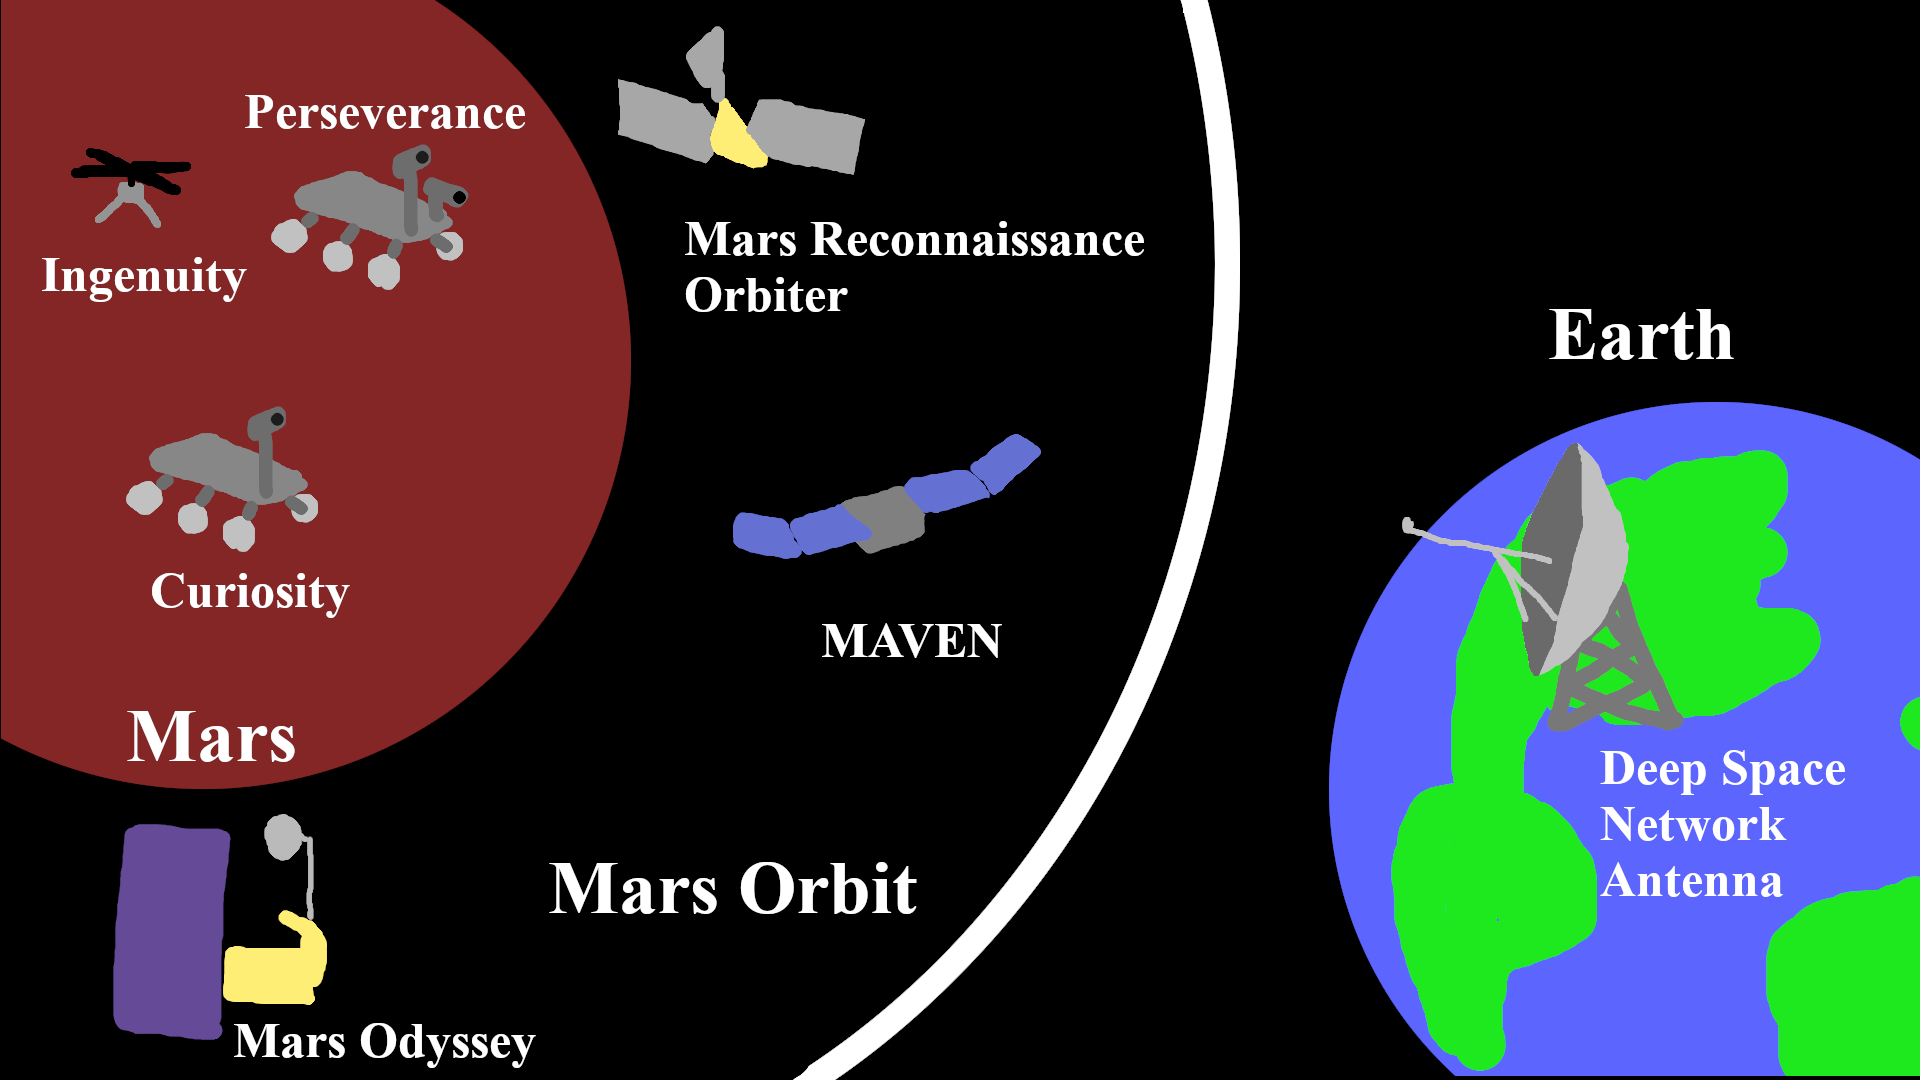
\includegraphics[width=\textwidth]{media/ipn.png}
  \caption{A sample of the current interplanetary network}
\end{figure}


To combat these challenges several protocols have been created. The SCPS TP is a
transport protocol which is used on the network layer. UDP is used in the lowest
reliable connections between nodes, and TCP is used in the most reliable network
conditions. When a reliable and efficient method of network transportation is
needed, then SCPS TP is used. It is a modified version of TCP which uses a slow
start protocol, reduced handshakes, reliable data transfer with reduced
confirmations. Other protocols like store and load, and Licklider are used to
also overcome these problems. In this paper since no complete implementation of
SCPS TP has been created for NS-3, New Reno TCP was used instead.

The rest of the paper remains to simulate these unique challenges, as well as
see how protocols operate at these different situations.

\section{Methodology}

\subsection{Physics Engine}

A significant challenge in modeling a IPN is modeling the rapidly changing
topology. To simulate these rapid changing conditions a physics engine was
created to model the orbits of several entities in the solar system. Several
assumptions were made in the simulator for the sake of simplicity as the goal of
the simulator is not to create a perfect model of the solar system and the
entities inside of the solar system, but rather conditions which a IPN would
exist in.

The first assumption made was that all orbits are circular. Realistically,
orbits are oval shaped, with two focal points. A result of this assumption is
the elimination of any difference in orbital speed due to Kepler's second law.
Normally a planet will accelerate or decelerate depending on where it is in its
orbit around the sun. The orbital radius was chosen by taking the average
orbital radius of the real life celestial bodies. For example Earth's average
orbital radius is 149.6 billion meters~\cite{nasa_earth}, and therefore orbits
around the sun in a circular orbit of radius 149.6 billion meters in our model.
Another result of this assumption is that orbits are considered to be centered
around the body which it orbits. The Mars orbit has a focal point that is
further in space, making it more oval shaped than the earth
orbit.~\cite{nasa_mars} While this could make changes to a simulated network in
some very specific situations, the primary behaviour of a solar system is
maintained, like retrograde orbits, periodical alignment, predictable behaviour,
and recursive orbits of sub orbiting object.

All entities are assumed to have a circular shape, with a constant radius. Due
to the scale of the objects, both large and small, this has a very minor effect.

The whole physics simulation has been done on a 2D plane. While planetary orbits
were not perfectly aligned, on the astronomical scale which we are working on,
assuming that all their orbits are contained on the same plane will not effect
the simulation significantly. Where this could be an issue is for when there are
more than two satellites orbiting the same entity, with a relatively low orbit.
For example satellites orbiting Earth. While there are some complex satellite
interactions which are removed it does still simulate satellites having to form
a network around the entity it is orbiting, it just requires less satellites
then if it needed to form a 3-D network.

Messages between entities were assumed to be sent at the speed of light in a
vacuum, as all forms of radio, lasers, or other wireless messages are forms of
electromagnetic radiation, and thus travel at the speed of light. Since the
propagation delay in an IPN is much higher than in terrestrial networks, other
delays such as processing delays were ignored as being negligible.

Based on these simplifications, a physical simulation with several goals. To
calculate if a line of sight could be made between two communicating entities,
that is if a message can be sent, to calculate the error rate when sending a
message, and to calculate the message propagation delay for the message to be
sent. Line of sight was achieved using simple geometry calculations. All
entities are able to block signals if the ray passes through the radius of the
entity. One of the largest factors contributing to transmission error is the
distance traveled by the electromagnetic signal between transmitting and
receiving nodes. By generalizing Friis' transmission formula\cite{Friis} for
isotropic emitters and receivers, we can obtain the ratio of signal intensity
received to signal intensity transmitted, known as Free Space Path Loss (FSPL).
We can use FSPL as our transmission error rate, giving the following expression:
$Error Rate = {(\frac{4 \pi d}{\lambda})}^2$ where $d$ is the distance between
nodes in metres and $\lambda$ is the wavelength of the electromagnetic wave used
in transmission. As much of space communications utilizes the Ka-band of
frequencies (27--40 GHz)\cite{Morabito_Hastrup} we opted to use a transmission
frequency of 30Ghz. The transmission wavelength can be then calculated according
to $\lambda = \frac{c}{f}$, where $c$ is the speed of light and $f$ is the
transmission frequency, giving a transmission wavelength of about 9.99~mm.
Propagation delay is a simple function of distance and the speed of light.

\begin{figure}[h]
  \centering
  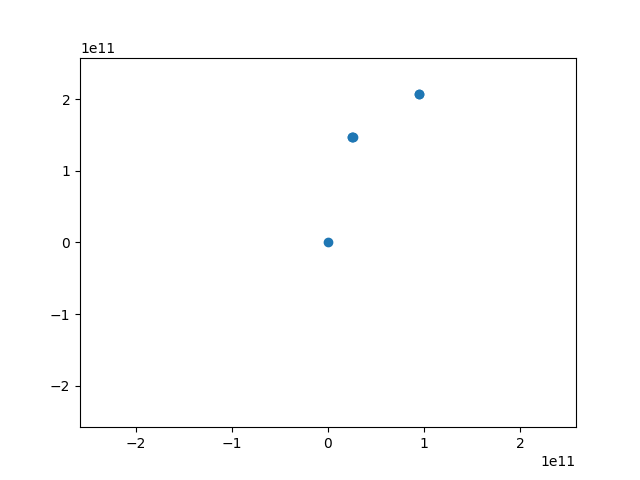
\includegraphics[width=0.4\textwidth]{media/sun_orbit.png}
  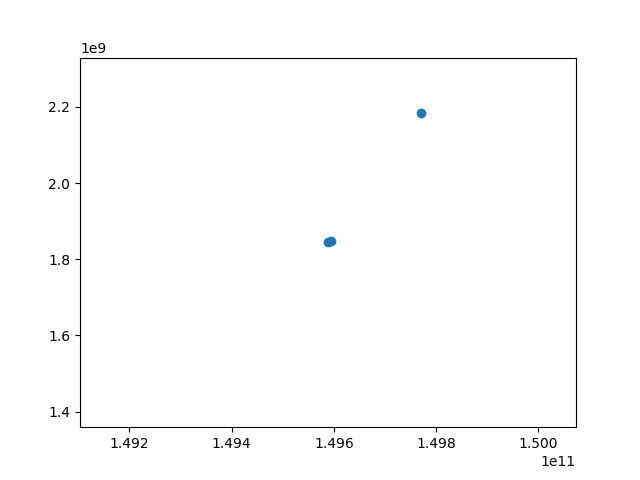
\includegraphics[width=0.4\textwidth]{media/moon_orbit.png}
  \caption{A visual output of the physics model. Left: Mars and Earth orbiting
    the sun. Right: The ISS (overlapping the center) and the Moon orbiting the
    Earth}
\end{figure}

The physics simulation modeled the Sun, Earth, Moon, International Space
Station, Mars, and the Mars Orbiter. All were able to connect to the network
except for the the Sun and the Moon. The input of the physics engine is a time
$t$ from some preset initial conditions which outputs the state of all entities.
Which is fed into the NS-3 simulation.

\subsection{Network Simulation}

We used NS-3~\cite{ns-3} to implement a simulation of this network. Our final
design consisted of a set of routers representing the different entities in our
physics simulation which were each linked to every other router using a
point-to-point channel. Essentially, this allowed us to have a wired network
with configurable delay and error along with the ability to take certain
channels down if they are obstructed that we could make behave like an
interplanetary network would without having to deal with the complexities of
configuring wireless communication. In addition to the mesh of routers, we added
two individual nodes to the network with zero delay that can be connected to any
one router in the network. One of these two nodes acts as a sender and the other
one acts as a receiver. This configuration of sender and receiver as separate
nodes made it easier to decouple the applications from the network topology and
allowed us to programmatically create arbitrary topologies.

NS-3 is a useful library, but we did run into a number of problems over the
course of our implementation of our simulation. The first problem came when we
first tried to compile the library itself and ran into a bug in the build script
that caused all executables to fail to run if there was the word ``scratch''
anywhere in the path due to a specific subdirectory of NS-3 which also happens
to be called ``scratch''. When first testing it out, one of us had put NS-3 into
a directory that happened to contain that word. We made a pull request to fix
this issue and it was merged by the NS-3 maintainers which allowed us to
continue.

The next issue we ran into was that we had decided to use the Python bindings to
allow us to easily use Python for the physics simulation. This was a mistake.
Although NS-3 does have Python bindings that do make it easier to run it as a
script after writing, there is no documentation at all for the Python bindings
and some basic features such as setting the error rate on a channel or
scheduling a task to run during the simulation have no Python support and must
use inline \CC. The lack of support for task scheduling in Python is
particularly bad as it forced us to schedule a \CC{} function which itself
called Python code. It also forced us to use global state as \texttt{CPyCpyy}
does not have support for arbitrary function parameters when calling Python code
as far as we could tell (this feature is not documented and we only figured out
about it because the few Python examples in the NS-3 source code that do use
scheduling also call Python from \CC{} with this method).

Before we settled on using point-to-point to emulate a wireless network, we
attempted to use the existing wireless networking features of NS-3. These
features are very powerful and even have a positioning and velocity system for
nodes in the network which would be very useful. We ran into a lot of issues
with this system though. Firstly, there only seems to be real support for Wi-Fi
which is not particularly useful for long distance unlike radio. This meant that
we would have to greatly decrease the distances that we were simulating. This is
fine and would still allow a perfectly reasonable simulation so long as we
increased the distances again in our computations while analyzing the data. The
other problem that we ran into is the fact that the wireless networking would
quickly require us to go well outside the scope of our project. Determining the
gain and energy required to configure our satellites to send and receive
messages correctly is more of an engineering problem that we were not interested
in solving.

After settling on using point-to-point, UDP was easy to get working but TCP
proved to be very challenging. Our initial implementation of our topology seemed
to have an issue where messages could be routed in one direction but not the
other. This meant that when TCP tried to establish a connection it would always
fail. It still is not entirely clear what was configured incorrectly, but after
changing how we were creating channels, TCP was finally working. We ran into
more issues with TCP though, when we started adding delay to the channels. It
turns out that NS-3 sockets have a rather low time-to-live and there do not seem
to be any global options for configuring sockets. We were left with two options:
implement TCP from scratch using custom-built sockets for each node in the
network or ensure that the messages that we do send have lower delay than the
TTL for our sockets. We opted for the latter. To make sure that TCP messages
could successfully ACK, we found a value that we could divide all times by to
make sure that almost every message that could feasibly be sent would be
received before its TTL expired. This does not change any distances or error
rates and effectively only changes the unit we use for time from $s$ to
$\frac{s}{26}$ which has an easy conversion back to $s$. Finally, we implemented
a version of our program using the New Reno variant of TCP. Thankfully, NS-3
made this easy for us. It worked perfectly after assigning a configuration value
before setting up our communication channels.

During the work on this project we contributed to the open source NS-3 project 
by committing a change to fix a bug which occurred when running the program on 
different operating systems.

\section{Data}
The NS-3 simulation ran on the basis of transferring data between Earth and 
Mars.

Data was scraped from the trace output that was generated while running the 
ns3 simulation. Trace data was given when a message was queued, dequeued, 
and received at the destination. This data also included the amount of 
data being sent in bytes. There is other data on the messages being sent, but 
was not tracked for the purpose of this project. The trace data was parsed 
using regex expressions to extract the needed numbers from the string.
This data was then fed into a pandas dataframe. A unique id had to be 
generated for each message since once a message was received the id was 
reused. This was done by tracking when each message was received with id 
$x$ and after incrementing a number by one, say $y$. The unique id was then 
created by hashing $xy$. Once the data frame was created it had to be merged 
on itself to have one row of the dataframe represent exactly one message rather 
then one row be either queue, dequeue, or received.

Time from being queued to received, time being queued, and message time in
transit were all calculated based off of the data.

\[\text{total\_package\_time} = \text{time\_recieved} - \text{time\_queued}\]

\[\text{time\_queued} = \text{time\_dequeued} - \text{time\_queued}\]

\[\text{total\_time} = \text{time\_received} - \text{time\_dequeued}\]

After the data was processed it was saved in a csv file with one row
representing exactly one message that was sent over the network. This file was
close to 2.5 GB in size.

Statistics were calculated on the entire column of the calculated rows, and
bytes sent. Messages were also grouped together which occurred during a similar
time window and further averages were calculated to find how the average changed
over time of the simulation. These calculations are shown in the graphs in the
analysis section.

\section{Analysis}

\subsection{UDP}

\begin{figure}[h]
  \centering
  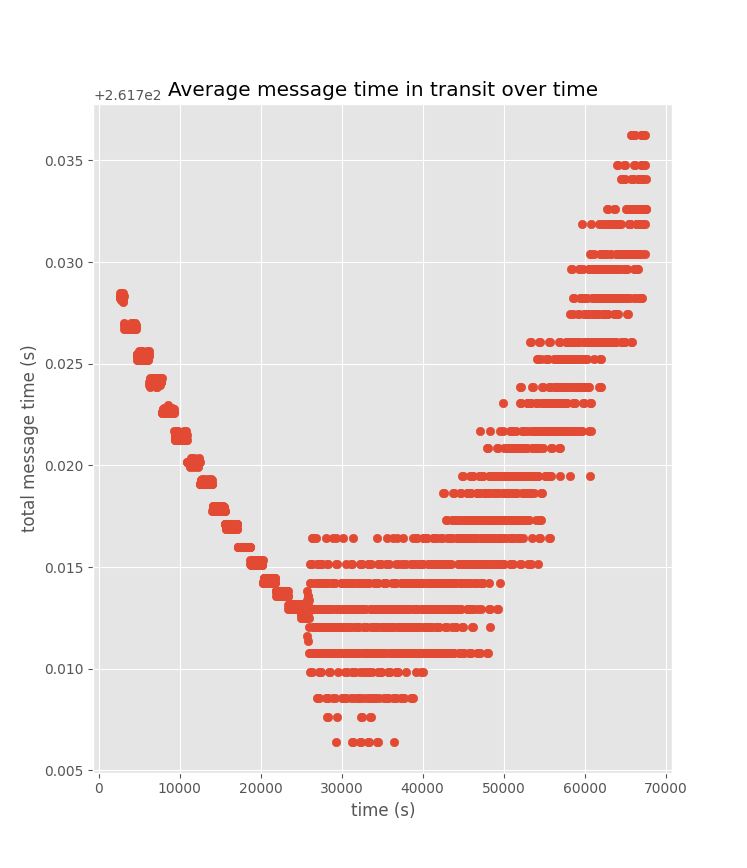
\includegraphics[width=0.4\textwidth]{media/udp.png}
  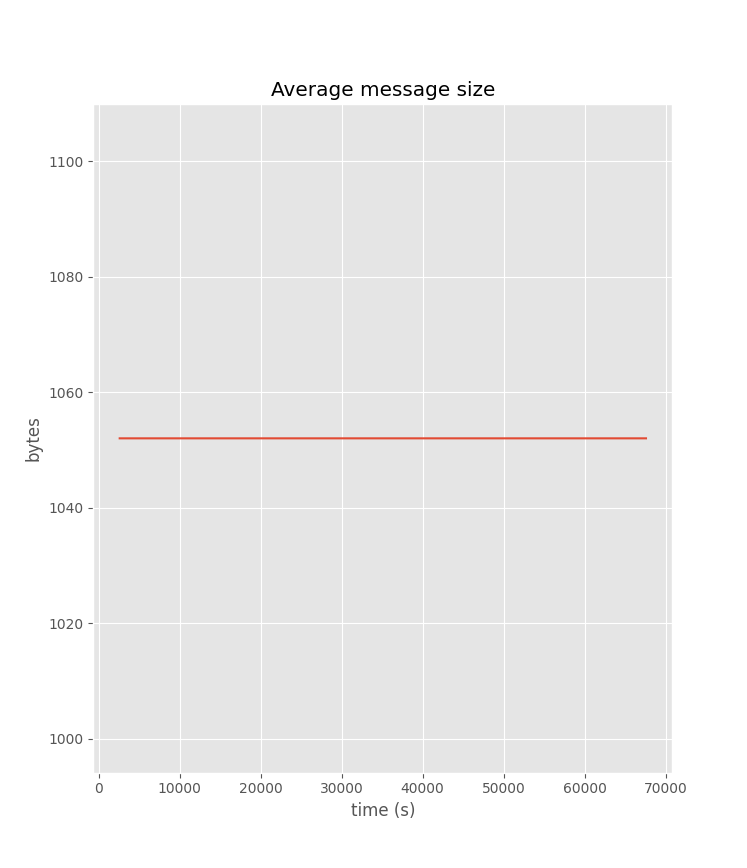
\includegraphics[width=0.4\textwidth]{media/udp_data.png}
  \caption{UDP analyzed}
\end{figure}

UDP had an average time from being queued to received of 283.64 seconds, an
average time being queued of 21.92 seconds, and an average message time in
transit 261.72 seconds. The average amount of data sent was 1052.0 bytes. Notice
the scientific notation in the corner of the graph.

The message size is the same across all of the messages. This makes sense as the message size do not need to be different across different messages. This is different compared to TCP and New Reno.

On the left side of the graph before approximately $t = 25000$ this is where
the planet most likely has a direct path between Earth and Mars. This has a
steady pattern of a batch of messages are queued, they are sent, and after they
are sent the next batch of messages are queued, and calculated the propagation
delay at the time that it is queued. This leads to the clusters which can be seen.
The curvature of the delay is most likely attributed to the movement of Earth
relative to Mars, that is that they are getting closer together. Queueing delay is likely small in this section suggested by the tight groupings.

At approximately time $t = 25000$ the direct path between Earth and Mars is
blocked. This means that the messages have to be routed through a secondary
satellite. The vertical gap between the horizontal lines is roughly 0.001
seconds. This is the same time as it takes for a message to take for a message
to send between Earth and the ISS and similarly between Mars and the Mars
Orbiter. The reason for the multiple horizontal lines is that messages may be
passed several times between the planet and its satellite before it is finally
delivered across the large propagation delay between the planets Earth and Mars.
The propagation delay could be seen through the length of the horizontal lines.
This is representative of the time it takes to clear each batch when it is sent.
Once an entire batch is sent it will re-calculate the propagation delay which
will then be represented in new different horizontal lines. The long lines show
that there was a large spike in queuing delay as the topology changed which
became smaller as it cleared. The curvature of this curve likely represents the
change in the relative distance between the satellites orbiting Earth and Mars
becoming further apart. This is clear here due to the extremely small variation
in propagation delay.

This analysis cannot be 100\% verified due to the data mined from NS-3 did not give a ton of information about the messages which were sent on our simulated network.

\subsection{TCP}

\begin{figure}[h]
  \centering
  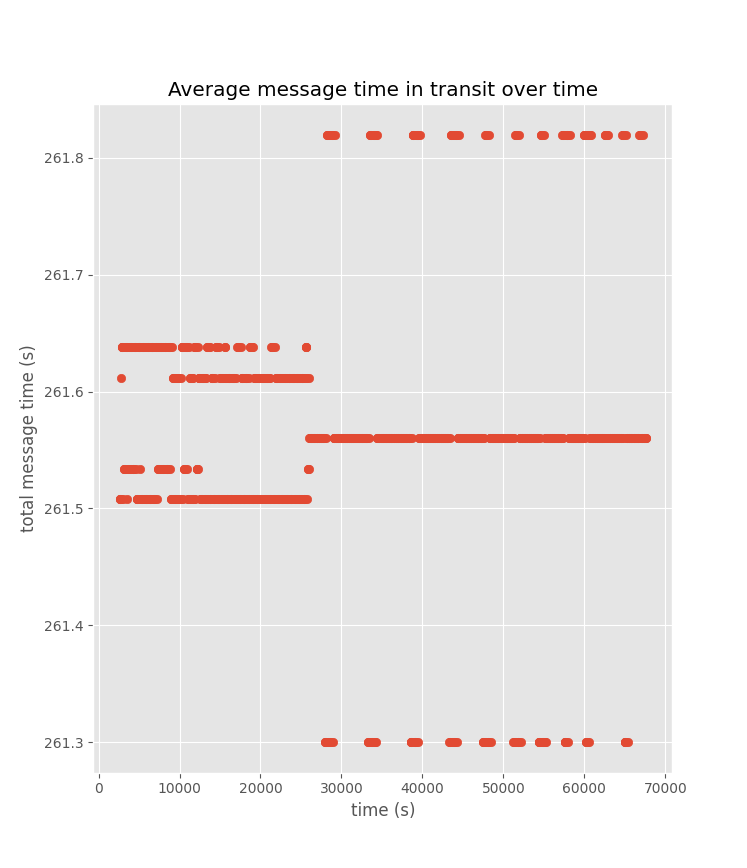
\includegraphics[width=0.4\textwidth]{media/tcp.png}
  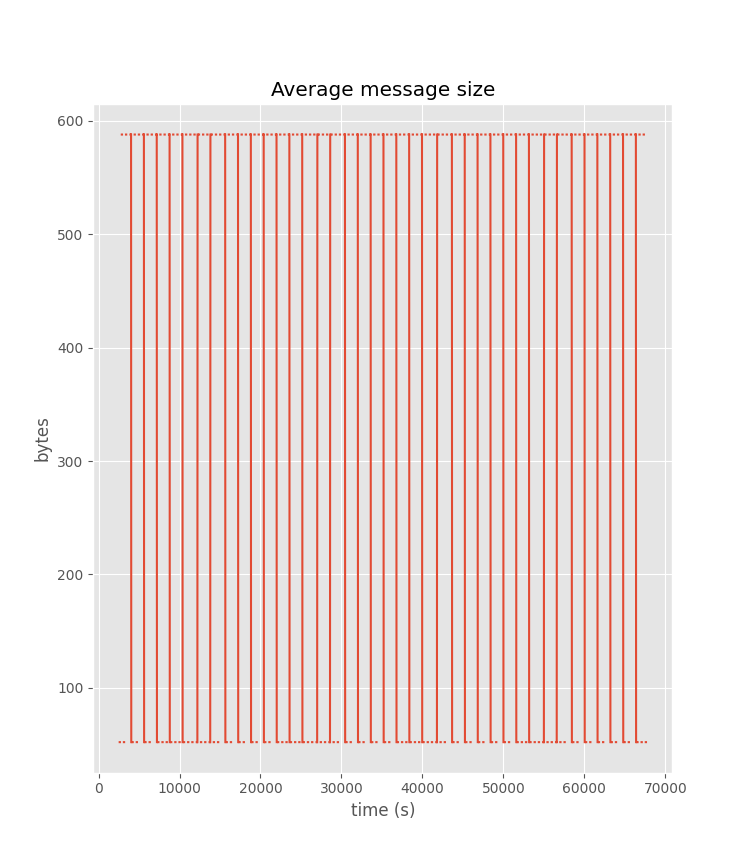
\includegraphics[width=0.4\textwidth]{media/tcp_data.png}
  \caption{TCP analyzed}
\end{figure}

The average amount of bytes transferred is 320.44 bytes. This is likely from the
difference in the amounts of bytes transferred in an ACK message compared to
when data is being sent.

Unlike in UDP the motion of the planets is not observable in the graph. However
this is because there are several different paths which the TCP message could
have taken which can be seen. Since TCP requires a higher amount of base time to
establish a connection compared to UDP, this means that when it ``hops'' between
entities it adds a larger base time.

At the start of the time we can see 4 separate paths. This would be the
different times that it would take for any of the 4 paths between Earth and
Mars, that is Earth to the ISS to the Mars Orbiter then to Mars, Earth to the
Mars Orbiter to Mars, Earth to the ISS to Mars, and finally Earth to Mars. After
one of the entities is blocking a direct signal it becomes only that 3 of these
options possible, with likely only two actual paths being viable. With less
available bandwidth it becomes slower on average. Smaller time may also be
correlated to the minority of messages which were sent with a smaller message
size.

\begin{figure}[h]
  \centering
  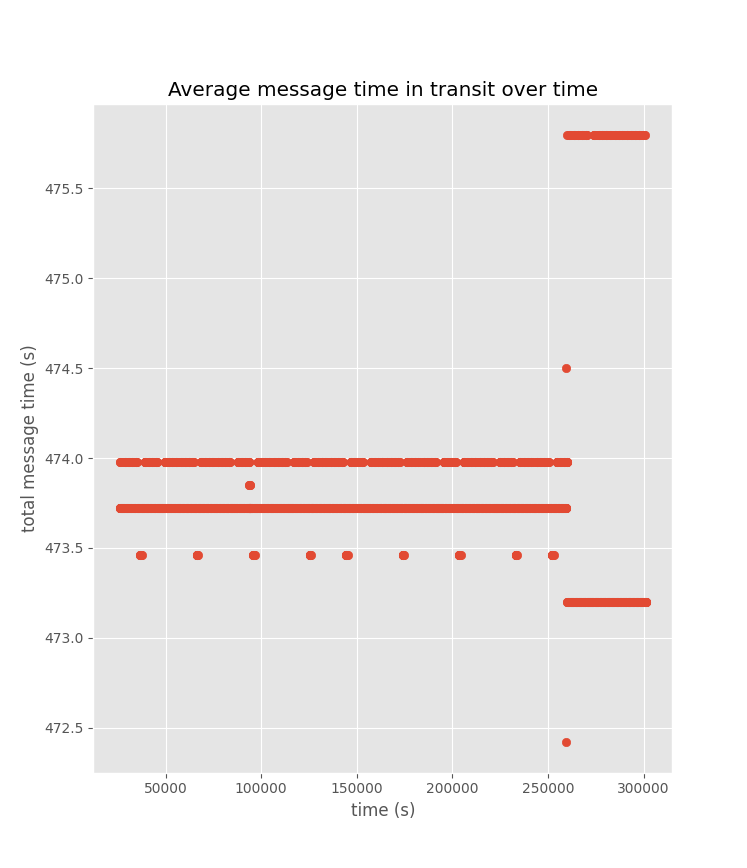
\includegraphics[width=0.4\textwidth]{media/tcp_future.png}
  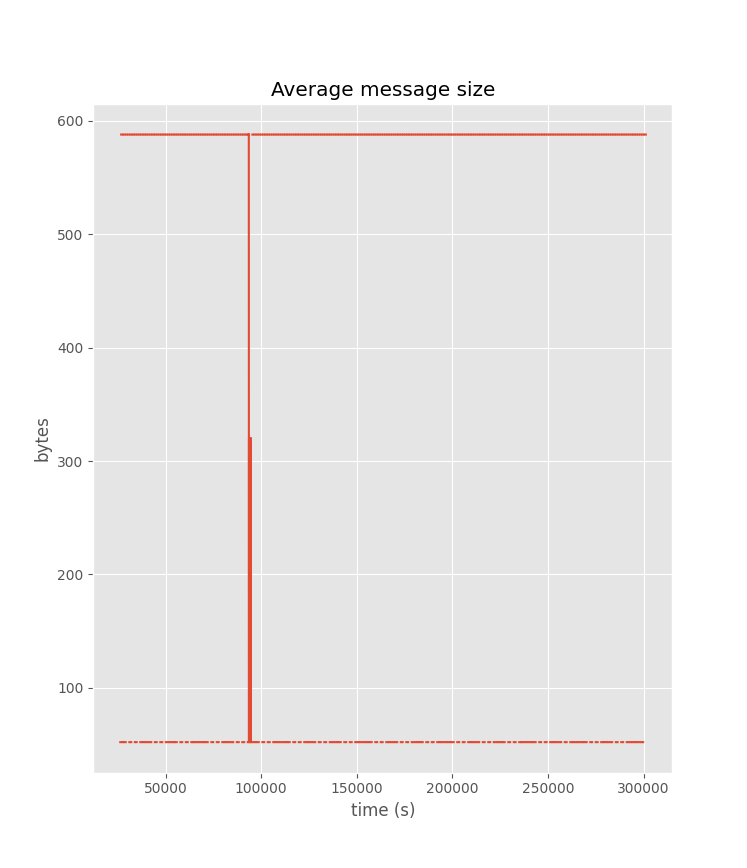
\includegraphics[width=0.4\textwidth]{media/tcp_future_data.png}
  \caption{TCP in the future analyzed}
\end{figure}

The second set of graphs show TCP in some time in the future. We can see that
the time that messages take to transfer does in fact change over time as the
entities change distances. We can also see a similar pattern of behaviour
changing as some topology changes in the model.

\subsection{New Reno}

New Reno, a modified version of TCP used to help reduce
congestion~\cite{Nahar2016}, was used in place of SCP TP. New Reno behaved very
similar to TCP. Its average data transfer was 307.18 bytes.

It preformed marginally better in its time from being queued to the message
received. This was mostly due to a decrease in time that it was in queue, which
is to be expected. There was a very marginal increase in time in transit
however.

\begin{figure}[h]
  \centering
  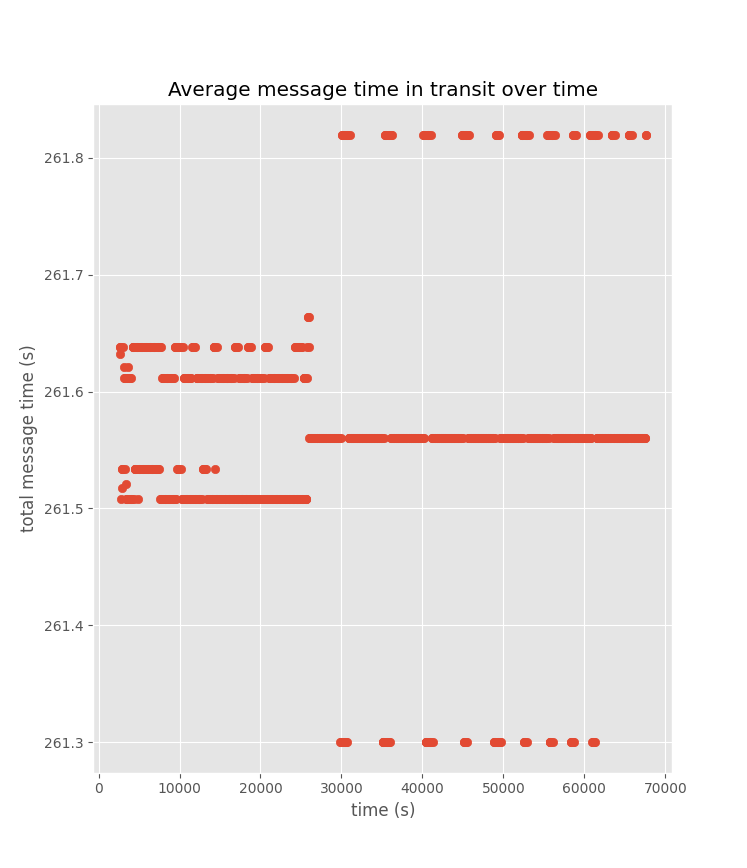
\includegraphics[width=0.4\textwidth]{media/new_reno.png}
  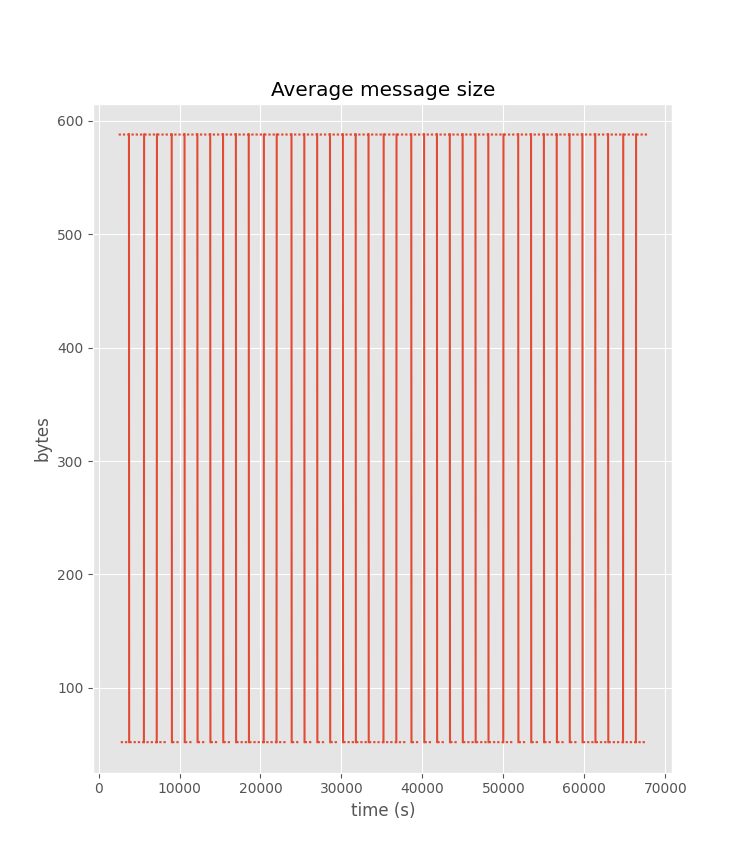
\includegraphics[width=0.4\textwidth]{media/new_reno_data.png}
  \caption{TCP in the future analyzed}
\end{figure}

Similar to TCP we can see the two stages which occur in the simulation. One
where most of the messages were likely being routed from directly from Earth to
Mars, which then gets transformed into having to route through one of the
external satellites orbiting each entity, which decreases the average time it
takes to transmit the message.

\subsection{Protocol Comparison}

Since a large amount of propagation delay dominates the amount of time that it
takes for messages total transmit time from being queued to being received at
the appropriate node, other increases in performance mean only a slight decrease
in time sending the message. An important statistic to pay attention to is that
UDP almost always sent a message with a size of 1052 bytes. This means that even
though TCP, New Reno, and UDP had sent a similar number of messages, the actual
throughput for UDP was significantly higher, which is much more significant in
an IPN situation. In the data graphs we can see that not only was the maximum
data being sent was less than UDP, but also had to send messages of very little
size, most likely acknowledgments, as well. New Reno was seen to improve on the
queuing time compared to both TCP and UDP. Which would mean in a high
reliability situation and in situations where higher traffic is sent through a
network with a relatively low bandwidth, like a IPN, where satellites are
limited by how much data they can transmit, New Reno's effect can be more
significant. This should only be used in a connection where propagation delay is
less of an issue like between planet and satellite communication. Queuing time
in UDP took a more significant percentage of its time than both TCP and New
Reno. In general however, UDP is the best option for primary communication
between Mars and Earth communication.

\section{Future Work}

Future work that could be done would be to implement or partially implement SCP
TP as a network protocol which could be used and compared to the protocols
analyzed in this paper. Other protocols like the Linklider or load and store
protocols could also be implemented, to create a more realistic IPN.

The physics engine could be expanded to included 3-D orbits, particularly around
planets, where networks of satellites could be created to create a proper level
of communication that is maintained today, with geocentric and polar orbiting
satellites. Connection points from a planet to off the planet could have a
direction which it needs to send a message in for it to be able to connect. For
example a rover on Mars in our simulation could technically send a message in
any direction, even if they were sending it through the surface of the
planet.The error model in the physics engine could be expanded to include
interference like solar radiation, atmosphere, and other interference.

Other stats could be extracted from the NS-3 model such as packet loss, message
path, handshake time. It could expand so that the network was not just focused
on Earth to Mars communication. It could be expanded to include other celestial
objects in the solar system, as well as potential future objects.

The NS-3 simulation could dynamically choose the network protocol to use based
on the level of error, message size, estimated propagation error, and other
factors. This could build a model which uses not only one protocol but all of
them and leverages the advantages of each when it is necessary. This combined
with a more sophisticated model of the solar system would create a very
competent simulation of the current operation of the IPN, and could then be
expanded or tweaked to find if expansions to it could be handled properly. This
would need a combination of all of the suggestions above to be successful.

\section{Conclusion}

In this paper we outlined how we created a model of an interplanetary internet
(IPN) using a physics engine which fed into a NS-3 simulation. The physics
simulation used a simplified model of orbiting planets and satellites as well as
physics calculations to create data which would be the output for any input time
$t$. The NS-3 model used a point to point base which programmatically took the
data from the physics engine and created nodes which acted as routers. A
simulation was ran which transferred data between Earth and Mars, using
satellites and other entities to relay messages around blocked connections.
Analysis was done on three different network protocols used in the IPN, that is
UDP, TCP and New Reno. UDP was found to have the most throughput out of all of
the three protocols, while New Reno reduced the amount of time a message was
queued.

\printbibliography{}

\end{document}
